\documentclass[11pt]{article}

\usepackage{../ppackage}
\usepackage{bbm}
\usepackage{import}






\usepackage{tikz}
\usetikzlibrary{arrows.meta,patterns}
\usetikzlibrary{ipe} % ipe compatibility library

\usepackage{../../../Notes/tikzit}
\usepackage{../../../Notes/utf8math}
\usetikzlibrary{positioning, 
                quotes}

\input{../../../Notes/TIKZ/digraph.tikzstyles}



\usepackage{url}


\newcommand{\solution}{
\bigskip\noindent
	\textbf{Solution: \\}}
	


\DeclareMathOperator{\size}{size}
\DeclareMathOperator{\conv}{conv}
\newcommand{\SV}{\mathrm{SV}}
\newcommand{\bigO}{O}
\newcommand{\cut}{\mathrm{cut}}
\newcommand{\LLL}{\mathrm{LLL}}
\newcommand{\setR}{\mathbb{R}}
\newcommand{\setZ}{\mathbb{Z}}
\newcommand{\setQ}{\mathbb{Q}}
\newcommand{\setC}{\mathbb{C}}
\newcommand{\setN}{\mathbb{N}}
\newcommand{\wt}[1]{\widetilde{#1}}
\newcommand{\opt}{{\sc 0/1-opt}\xspace}
\newcommand{\aug}{{\sc 0/1-aug}\xspace}
\newcommand{\psep}{{\sc 0/1-psep}\xspace}
\newcommand{\sep}{{\sc 0/1-sep}\xspace}
\newcommand{\fopt}{{\sc 0/1-testopt\xspace} }

\newcommand{\hpp}{\mathrm{HPP}}
\newcommand{\nodes}{\mathcal{V}}
\newcommand{\vol}{\mathrm{vol}}
\newcommand{\diag}{\mathrm{diag}}
\newcommand{\arcs}{\mathcal{A}}
\newcommand{\edges}{\mathcal{E}}
\newcommand{\paths}{\mathscr{P}}
\newcommand{\cycles}{\mathcal{C}}




\newcommand{\K}{{\mathcal K}}
\newcommand{\A}{{A}}
\newcommand{\B}{{B}}
\newcommand{\T}{\mathscr{T}}
\newcommand{\eE}{\mathscr{E}}
\newcommand{\eS}{\mathscr{S}}
\newcommand{\eP}{\mathscr{P}}
\newcommand{\eM}{\mathscr{M}}



\newcommand{\transp}{^{\mathrm{T}}}

\newcommand{\smallmat}[1]{\left( \begin{smallmatrix} #1 \end{smallmatrix}\right)}

\newcommand{\mat}[1]{ \begin{pmatrix} #1 \end{pmatrix}}
\newcommand{\smat}[1]{ \big(\begin{smallmatrix} #1 \end{smallmatrix}\big)}

\newcommand{\pc}{\mathscr{P}}
\newcommand{\ob}{\mathscr{O}}
\newcommand{\odds}{\mathscr{W}}
\newcommand{\up}{\mathscr{U}}
\newcommand{\ef}{\mathscr{F}}
\newcommand{\eh}{\mathscr{H}}
\newcommand{\ev}{\mathscr{V}}
\newcommand{\ec}{\mathscr{C}}
\newcommand{\eu}{\mathscr{U}}

\newcommand{\lex}{\mathrm{lex}}

\renewcommand{\leq}{\leqslant}
\renewcommand{\geq}{\geqslant}









\newcommand{\linhull}{\mathrm{lin.hull}}
\newcommand{\affhull}{\mathrm{affine.hull}}
\newcommand{\charcone}{\mathrm{char.cone}}
\newcommand{\cone}{\mathrm{cone}}
\newcommand{\rank}{\mathrm{rank}}
\newcommand{\wb}[1]{\overline{#1}}



\usepackage{enumerate}

      
\institute{\'Ecole Polytechnique F\'ed\'erale de Lausanne}
\lecture{Discrete Optimization}
\faculty{Prof. Eisenbrand}
\term{Spring 2025}
\publishdate{May 6, 2025}
\duedate{ }
\problemset{Assignment~11}

\begin{document}
\makeheader

\begin{enumerate}[1)]
\item Find a maximum cardinality matching and a minimum cardinality vertex cover in the following graph.
  \begin{center}
    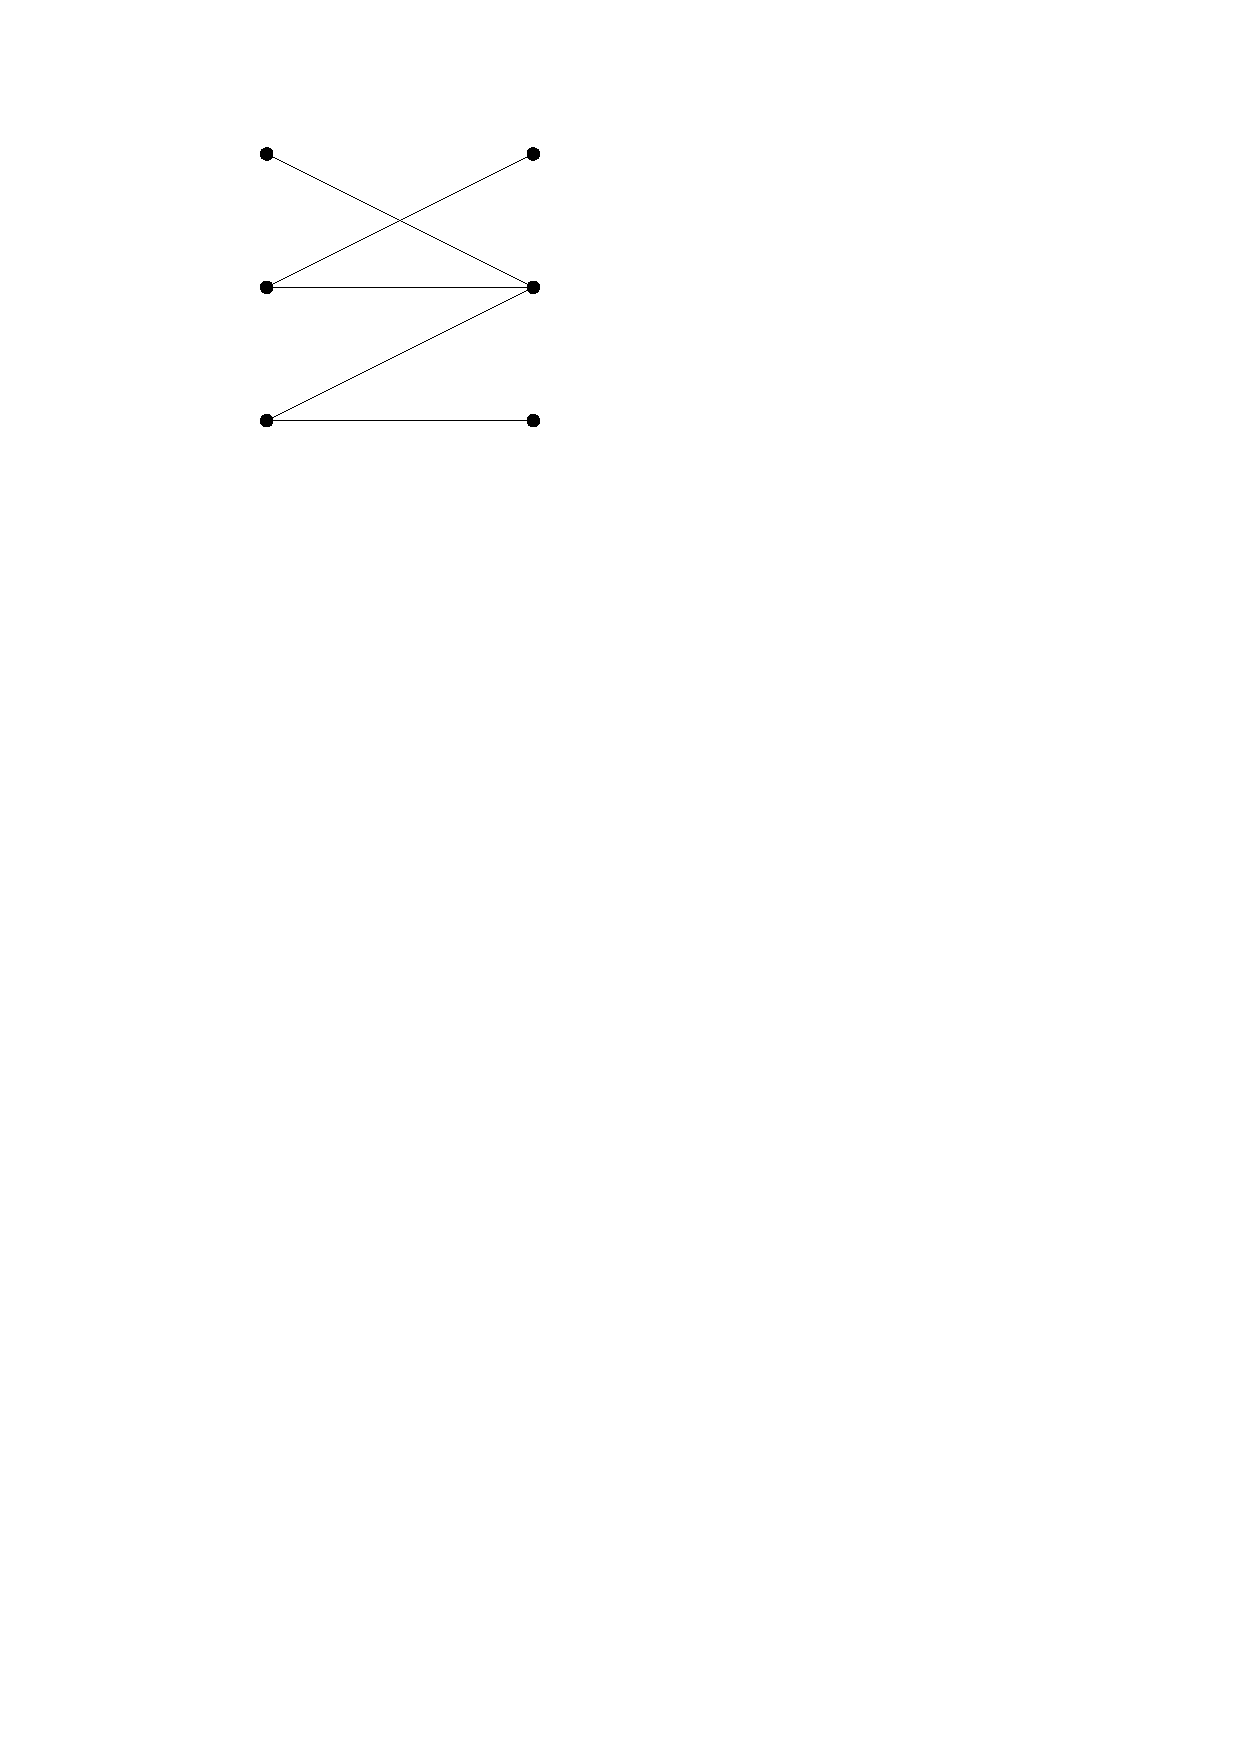
\includegraphics[width=0.2\textwidth]{../graph1}
  \end{center}
  
  
  
  \begin{solution}
  We match the nodes as follows using the red colored edges to give a maximum matching and give a minimum vertex cover by the blue shaded nodes. Clearly both have size 3. 
  
  \begin{figure}[h!]
    \centering
    \begin{tikzpicture}[node distance=2cm,
    B/.style={circle, draw, minimum size=.1cm},A/.style={fill=blue!50, circle, draw, minimum size=.1cm},
    edge/.style={->,> = latex', font=\footnotesize}]
    
    \node[B] (s) at (0, 0) {};
    \node[A](a) at (3, 0){};
    \node[B](c) at (0, -1.5){};
    \node[B](b) at (0,-3){};
    \node[A](d) at (3, -1.5){};
    \node[A](t) at (3, -3){};
    
    
    %\draw[color=red, line width=2.0pt] (s)--(d);
    \draw[color=red, line width=2.0pt] (s)--(d);
    \draw [color=red, line width=2.0pt](c)--(a);
    \draw (c)--(d);
    %\draw (c)--(t);
    \draw (b)--(d);
    \draw[color=red, line width=2.0pt] (b)--(t);

    




    
    %\draw (s) -- (a) node[midway, fill=white]{$7/10$};
    %\draw (s) -- (c){$8/10$};
    %\draw (a) -- (c){$0/4$};
    %\draw (c) -- (a){$2/5$};    
    
    
    
    \end{tikzpicture}
    \end{figure}
    
    \end{solution}
  
  
  
\item 
Let $A \in \R^{n \times n}$ be an invertible matrix and $b \in \R^{n}$ a vector. The ellipsoid $E(A,b)$ is defined as the image of the unit ball under the linear mapping $t(x) = Ax+b$. Show that
$$E(A,b) = \{ x \in \R^n: (x-b)^\top A^{-\top} A^{-1} (x-b) \leq 1 \}.$$


\begin{solution}
The ellipsoid $E(A,b)$ is the image of the unit ball by a linear mapping $t(x) = Ax+ b$. The unit ball
is denoted by $B(0,1) := \{x∈\setR^2 : \Vert x\Vert_2^2 ≤1\}$. Hence,
\begin{align*}
E(A,b) &= \{t(x) ∈\setR^2 : \Vert x\Vert^2_2 ≤1\} \\
& = \{Ax+ b∈\setR^2 :\Vert x\Vert_2^2 ≤1\} \\
& = \{y∈\setR^2 :\Vert A^{-1} (y−b)\Vert_2^2 ≤1\}\\
&= \{y∈\setR^2 :(y−b)^T A^{−T} A^{-1}(y−b) ≤1\}.
\end{align*}
\end{solution}
	
\item 
Draw $E(A,b)$ for $A = \begin{pmatrix} 1 & 3  \\ 2 & 5 \end{pmatrix}$ and $b  = \begin{pmatrix} 1   \\ 2 \end{pmatrix}$. What are the axes of $E(A,b)$?


\begin{solution}
Using the previous exercise, we have that $E(A,b) = \{x∈\setR^2 : (x−b)^TA^{-T}A^{-1}(x−b) ≤1\}$. From
linear algebra, the matrix $A^{-T} A^{-1}$ is symmetric, in particular has real eigenvalues and is diagonalizable by an orthogonal matrix $S$, i.e. $A^{-T} A^{-1} = SDS^T$ , where D is diagonal.
So we can rewrite $E(A,b) = \{x∈\setR^2 :(S^T(x−b))^T
·D·S(x−b) ≤1\}= \{x∈\setR^2 :λ_1\left(\frac{x_1-b_1}{c_1}\right)^2+  λ_2\left(\frac{x_2-b_2}{c_2}\right)^2  ≤1\}$,for $λ_1,λ_2$ diagonal elements of $D$, and $b_1,b_2,c_1,c_2$ determined by $S$. Therefore, the
eigenvectors of the matrix $A^{-T}A^{-1}$ define the principal directions of the ellipsoid and the square
root of the corresponding eigenvalues determines their length.
For our example we have $v_1 ≈(3.17,5.38)$ and $v_2 ≈(−0.14,0.08)$ with $λ_1 = 39$ and $λ_2 = 0.026$.
\end{solution}

\item Let $D = (V,A)$  be a directed graph and $A_D ∈ \{0,\pm1\}^{|V| × |A|}$ be the node-edge incidence matrix of $D$. Assume that the underlying undirected graph $G = (V,E)$  with $E = \{ uv : uv ∈A \text{ or } vu ∈ A\}$ is connected. 
  \begin{enumerate}[i)]
  \item Show that any row of $A_D$ is in the span of the other rows.
  \item Let $T ⊆ A$ be a selection of $n-1$ arcs of $A$ such that the induced undirected graph is a spanning tree of $G$. Show that the corresponding columns of $A_D$ are linearly independent.
  \end{enumerate}
  
  
  \begin{solution}
  
  \begin{enumerate}[i)]
  \item Sum up all of the rows in $A_D$. Since every column corresponds to a directed edge, the column has exactly one $+1$ entry corresponding to the incoming node and one $-1$ entry corresponding to the outgoing node. Thus summing all rows gives the all zeros vector which means that any row is in the span of the other rows. 
  
  \item We proceed by induction on $n$:

Base case: $n=2$ is true trivially. 

Suppose it is true for a tree on $n$ nodes then let $T$ be a tree on $n+1$ nodes. Let the incidence matrix of $T$ have columns $c_1, \hdots, c_{n}$. I.e. for $n+1$ nodes there are $n$ edges of the spanning tree so $n$ columns of the incidence matrix. 
Without loss of generality, we assume column $n$ represents an edge attached to a leaf. (say node $v_{n+1}$ is a leaf). Removing node $v_{n+1}$ (thus edge $e_n$) gives another tree on $n$ nodes with incidence matrix of columns $c_1, \hdots, c_{n-1}$. 

By induction, this smaller incidence matrix has linearly independent columns. Adding back $v_{n+1}$ we get back our original incidence matrix. let
$a_1c_1+...+a_{n−1}c_{n−1}+a_nc_n=0$ such that the full set of columns of $T$ are not linearly independent. \\
Case 1: $a_n=0$ then by linear independence of $c_i$ for $i≤n−1$ we must have $a_i=0$ for $i≤n−1$.

Case 2: $a_n\neq 0$ then
$a_1c_1+...+a_{n−1}c_{n−1}=−a_nc_n⟹b_1c_1+...b_{n−1}c_{n−1}=c_n$
where $b_k= - \frac{a_k}{a_n}$. Thus $c_n$ is linear combination of columns of the smaller spanning tree. This gives a contradiction since $c_n(v_{n+1})=1$ since the final edge is incident to node $v_{n+1}$ and as the degree of $v_{n+1}$ is $1$ in $T$, column $c_n$ is the only column with nonzero entry on row $n+1$. 
  
  \end{enumerate}
  \end{solution}
  
  
  
\item Let $f \in \mathbb{R}^{|A|}_{\geq 0}$ be a flow of a directed graph. Show that we can find a feasible flow $f^*$ such that $f^* = \sum_{p \in P}  \mu_p \cdot p + \sum_{c \in C}\mu_c \cdot c$ where $C$ is a set of cycles in the graph, $P$ is a set of paths in the graph, and $\mu_l, \mu_p \in \mathbb{R}_{\geq 0}$.

\medskip 

\paragraph{Example:}

\begin{figure}[h!]
    \centering
    \begin{tikzpicture}[scale=1.5,node distance=2cm,
    B/.style={circle, draw, minimum size=.8cm},
    edge/.style={->,> = latex', font=\footnotesize}]
    
    \node[B] (s) at (0, 0) {$s$};
    \node[B](a) at (2, 1){$a$};
    \node[B](c) at (2, -1){$c$};
    \node[B](b) at (4, 1){$b$};
    \node[B](d) at (4, -1){$d$};
    \node[B](t) at (6, 0){$t$};
   \node (a2) at (2.1, 0.75){};
   \node (c2) at (2.1, -0.75){};
   \node (b2) at (4.1, 0.75){};
   \node (d2) at (4.1, -0.75){};
    
    \draw[edge] (s) to node[above left ] {$7/10$} (a);
    \draw[edge] (s) to node[below left ] {$8/10$} (c);
    \draw[edge] (a2) to node[right] {$2/5$} (c2);
    \draw[edge] (c) to node[left] {$0/4$} (a);
    \draw[edge] (a) to node[above ] {$5/5$} (b);
    \draw[edge] (b) to node[above ] {$0/7$} (c);
    \draw[edge] (b2) to node[ right ] {$2/6$} (d2);
    \draw[edge] (c) to node[below ] {$10/10$} (d);
    \draw[edge] (d) to node[ left ] {$0/10$} (b);
    \draw[edge] (b) to node[above ] {$3/3$} (t);
    \draw[edge] (d) to node[below ] {$12/14$} (t);
    




    
    %\draw (s) -- (a) node[midway, fill=white]{$7/10$};
    %\draw (s) -- (c){$8/10$};
    %\draw (a) -- (c){$0/4$};
    %\draw (c) -- (a){$2/5$};    
    
    
    
    \end{tikzpicture}
    \end{figure}
    
    
    

This flow can be decomposed into the following combination of paths:\\
•$p1: s →a →b →t$ ($f1$ assigns $3$ units to each edge in $p1$)\\
•$p2: s →c →d →t$ ($f2$ assigns $8$ units to each edge in $p2$)\\
•$p3: s →a →b →d →t$ ($f3$ assigns $2$ units to each edge in $p3$)\\
•$p4: s →a →c →d →t$ ($f4$ assigns $2$ units to each edge in $p4$)


\begin{solution}
Given network with a feasible flow $f$ we construct the following procedure to get $f*$:
\begin{enumerate}
\item Find $Γ$, any path or cycle with unequal flow values on its edges.
\item Let the flow quantity of $Γ$ be the minimum flow on any edge of $Γ$. Reduce the flow on every edge of $Γ$
by that quantity. Return to step 1.
\end{enumerate}
Step $2$ reduces flow until it completely removed flow from at least one edge of $Γ$. Thus the algorithm continues while any path or cycle has unequal flow values and must terminate if the entire network has flow value $0$, so that we eventually halt either with $0$ flow everywhere which is feasible for $f*$ or with a decomposition of flow as paths and cycles of equal flow value. These paths and cycles with equal flow value form our $f*$ with flow values $\mu_p$ and $\mu_c$ for the given paths and cycles.


\end{solution}



\item Let $D= (V,A)$ be a digraph. For every $a∈A$, let $l_a, u_a \in \mathbb{R}_{\geq 0}$ be given such that $l_a \leq u_a$. Show that
the set of circulations $\{x∈\setR^A : A_Dx= 0, l \leq x \leq u \}$ (with $A_D$ being the node-arc incidence matrix of $D$) is nonempty if and only if
$$ \displaystyle\sum_{a \in \delta^-(X)} l_a \leq \displaystyle\sum_{a \in \delta^+(X)} u_a \quad \text{for all }X \subseteq V. $$

\begin{solution}
We first prove the $\Rightarrow$ direction. Assume that the set of circulations is nonempty and let $x\in \mathbb{R}^A$ be such a circulation. Then for any $X\subseteq V$ we have 
\[
\sum_{a \in \delta^-(X)} l_a \leq \sum_{a \in \delta^-(X)} x_a = \sum_{a \in \delta^+(X)} x_a \leq \sum_{a \in \delta^+(X)} u_a,
\]
where the first and last inequality follows from $l\leq x\leq u$ and the equality in the middle follows from $A_D x=0$: for each node $v \in X$ we have $\sum_{a \in \delta^-(v)} x_a = \sum_{a \in \delta^+(v)} x_a$, summing them up over all $v\in X$ and cancelling common terms on both sides.

Next we prove the $\Leftarrow$ direction. For each $X\subseteq V$, define its slack $s(X):= \sum_{a \in \delta^+(X)} u_a - \sum_{a \in \delta^-(X)} l_a$.
Assume that $ \displaystyle\sum_{a \in \delta^-(X)} l_a \leq \displaystyle\sum_{a \in \delta^+(X)} u_a$ holds for all $X\subseteq V$, i.e., $s(X) \geq 0$ for all $X\subseteq V$. We will construct a circulation $x \in \mathbb{R}^A$. 
First if for all $a\in A$ we have $u_a=l_a$, then we claim that $x:=u=l$ is a circulation. Indeed, for any $v\in V$, we have 
\[
0\leq s(\{v\}) = \sum_{a \in \delta^+(v)} u_a - \sum_{a \in \delta^-(v)} l_a = \sum_{a \in \delta^+(v)} x_a - \sum_{a \in \delta^-(v)} x_a
\]
and
\[
0\leq s(V\setminus \{v\}) = \sum_{a \in \delta^+(V\setminus \{v\})} u_a - \sum_{a \in \delta^-(V\setminus \{v\})} l_a = \sum_{a \in \delta^-(v)} x_a - \sum_{a \in \delta^+(v)} x_a
\]
which implies that $\sum_{a \in \delta^+(v)} x_a - \sum_{a \in \delta^-(v)} x_a = 0$ for each $v\in V$, i.e., $A_Dx=0$.
Next we deal with the case when there exists $a\in A$ such that $u_a>l_a$. We will present a procedure, which increases $l_a$ and decreases $u_a$ so that eventually $u_a=l_a$, and at the same time maintaining the non-negativity of $s(X)$ for all $X\subseteq V$. Then by doing the procedure for each $a\in A$ with $u_a>l_a$ one at a time, we can reduce the problem to the case $u=l$ which we have solved.

The procedure is as follows. For any $a\in A$ with $u_a>l_a$, take $X\subseteq V$ to be the subset with the minimum slack such that $a\in \delta^{+}(X)$, and take $Y \subseteq V$ to be the subset with the minimum slack such that $a\in\delta^-(Y)$. 
Define $A^\prime \subseteq A$ to be all the arcs between $X\setminus Y$ and $Y\setminus X$. Note that $a \in A^\prime$. Then we have
\[
s(X) + s(Y) = s(X\cap Y) + s(X\cup Y) + \sum_{a^\prime\in A^\prime} (u_{a^\prime}-l_{a^\prime}) \geq u_a - l_a>0.
\]
Pick $\alpha, \beta\geq 0$ such that $\alpha+\beta = u_a-l_a$ and $\alpha\leq s(X), \beta\leq s(Y)$. Then we increase $l_a$ to $l_a+\beta$ and decrease $u_a$ to $u_a - \alpha$. By the minimality of $s(X), s(Y)$, the slacks of all subsets of $V$ are still non-negative.
\end{solution}

\end{enumerate}




  

\end{document}

%%% Local Variables:
%%% mode: latex
%%% TeX-master: t
%%% End:
